\documentclass[class=article , crop=false, titlepage, twoside, multi={itemize, figure, verbatim}, float=false]{standalone}

\usepackage{import} % Required for importing other .tex docs.  (import uses everything bw Begin and End Doc)
\usepackage{float} % Required for specifying the exact location of a figure or table
\usepackage{graphicx} % Required for including images
\usepackage{wrapfig}
\usepackage[pdftex,breaklinks,colorlinks=true,linkcolor=black,citecolor=blue,urlcolor=red,linktocpage=false,pagebackref=true,filecolor=magenta]{hyperref}%http://www.tug.org/applications/hyperref/manual.html#x1-100003.6
\usepackage{cite}
\usepackage[toc,title,page]{appendix}
\usepackage{pdfpages} % enables loading a pdf into the doc
\usepackage{makeidx}
\usepackage{glossaries} % must be after hyperref
\usepackage{blindtext}
\usepackage{enumitem}
%\usepackage{caption}

%\setlist[description]{leftmargin=\parindent,labelindent=\parindent}

%\renewcommand*{\bibname}{References} % renames the bibliography

\newcommand{\HRule}{\rule{\linewidth}{0.5mm}} % Command to make the lines in the title page

\graphicspath{{img/}{GIS_ChampionSection/img/}{awardsChapter/GIS_ChampionSection/img/}{brandPart/awardsChapter/GIS_ChampionSection/img/}{img/}{pairedProgSection/img/}{methodChapter/pairedProgSection/img/}{methodPart/methodChapter/pairedProgSection/img/}{documentationSection/img/}{methodChapter/documentationSection/img/}{methodPart/methodChapter/documentationSection/img/}{docStorageOrgSection/img/}{methodChapter/docStorageOrgSection/img/}{methodPart/methodChapter/docStorageOrgSection/img/}{QGisSection/img/}{toolsChapter/QGisSection/img/}{servicePart/toolsChapter/QGisSection/img/}{ESRISection/img/}{toolChapter/ESRISection/img/}{servicePart/toolChapter/ESRISection/img/}{../../../../source/}{../../source/}{servicePart/applicationsChapter/treasurerSection/img/}}

%\setlength\parindent{0pt} % eliminates indents


\def\titlename{Query Layers\\ \medskip\large Creating Queries in ArcGIS}

\title{\HRule % Horizontal Line added
\\[.4cm] % space
\begin{figure}[H] % included image
\begin{center}	% centered horizontally

\includegraphics[scale=.45]{GIS_Logo_better.jpg}
\end{center}
\end{figure}
\Huge \bfseries \titlename \\ % Title text
\HRule \\[.4cm] % Horizontal Line added
\author{\Large Allegan County GIS \\\Large www.allegancounty.org/gis} % defines author
}  % inputs common title
\setcounter{tocdepth}{5}  % subparagraph and down
\begin{document}% document begins
\ifstandalone
%\frontmatter % turns off chapter numbering and uses roman numerals for page numbers
\maketitle % creates title page and blank page after title page
\tableofcontents % creates TOC and blank page
\clearpage
%\mainmatter % turns on chapter numbering, resets page numbering and uses arabic numerals for page numbers
\fi

\subsection{Create Query in ArcGIS to SQL Database}
\medskip
\subsubsection[Add Query Layer ]{\Large Add Query Layer}
\paragraph*{In ArcMap: \texorpdfstring{\\}{}}
Open the New Qery Layer Dialog\\
Go to File Add Data Add Query Layer
In the connection dropdown select your connection
\paragraph*{}NOTE
\begin{figure}[h!]
\centering
    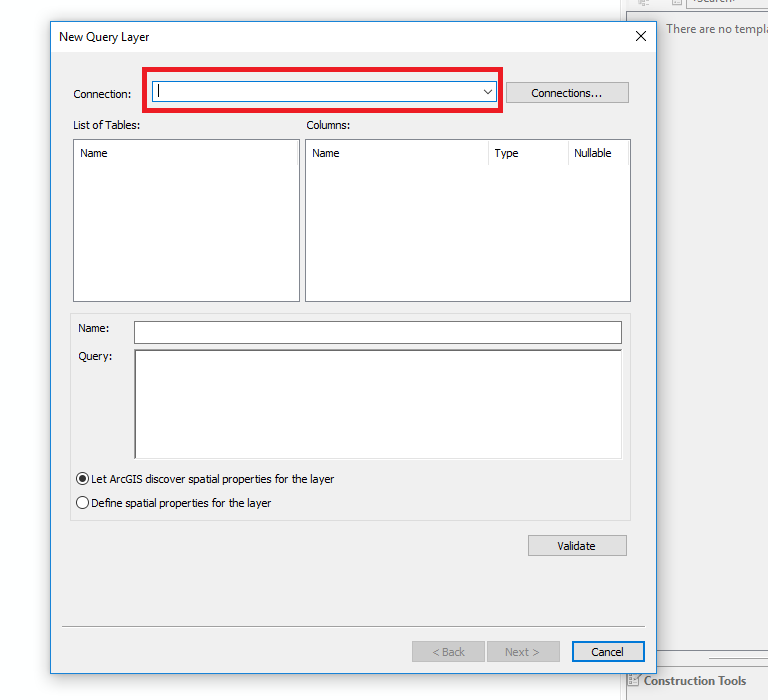
\includegraphics[width=.95\textwidth]{NewQueryLayerDialog.png}
\caption{New Query Layer Dialog}
\end{figure}
\clearpage
\subsubsection[Details of the Query Layer]{\Large Details of the Query Layer}
\paragraph*{Enter into the tool \texorpdfstring{\\}{}}
\begin{itemize}
  \item Choose connection
  \item Name the query
  \item Enter SQl query
  \item Press Next
\end{itemize}
\begin{figure}[h!]
\centering
    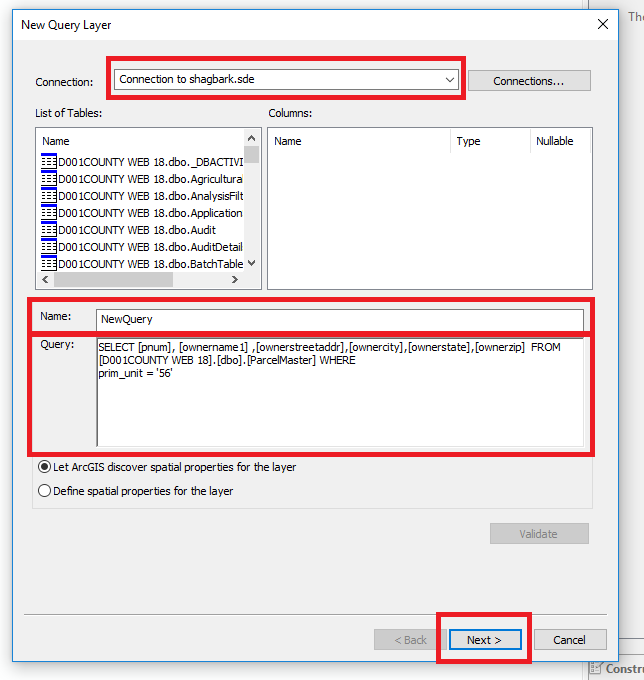
\includegraphics[width=.95\textwidth]{NewQueryLayerDialogFilled.png}
\caption{Query Layer Dialog Filled}
\end{figure}
\clearpage
\subsubsection[More Details of the Query Layer]{\Large More Details of the Query Layer}
\paragraph*{Enter into the tool \texorpdfstring{\\}{}}
\begin{itemize}
  \item Select unique identifier field
  \item Click Finish
\end{itemize}
\begin{figure}[h!]
\centering
    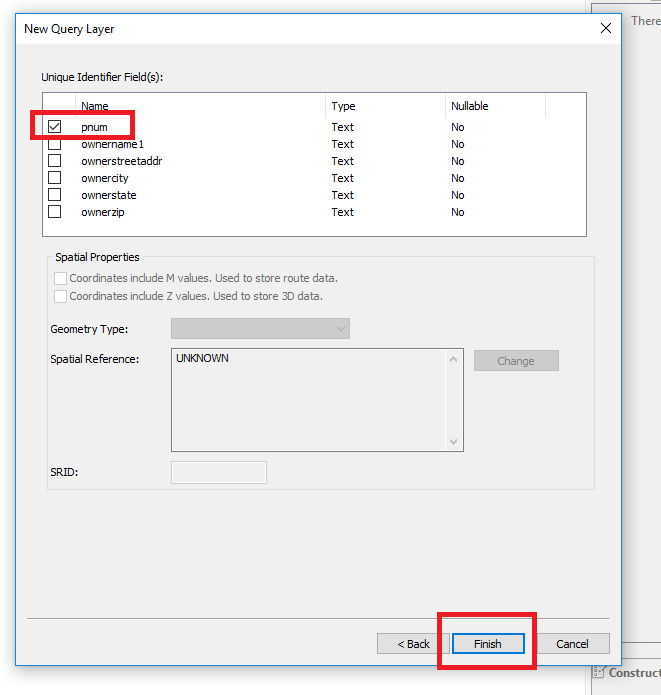
\includegraphics[width=.95\textwidth]{SelectUniqueIdentifier.PNG}
\caption{Select Unique Identifier}
\end{figure}
\clearpage
\subsubsection[Open Results Table]{\Large Open Results Table}
\paragraph*{Verify the Query by Looking at the Table \texorpdfstring{\\}{}}
\begin{figure}[h!]
\centering
    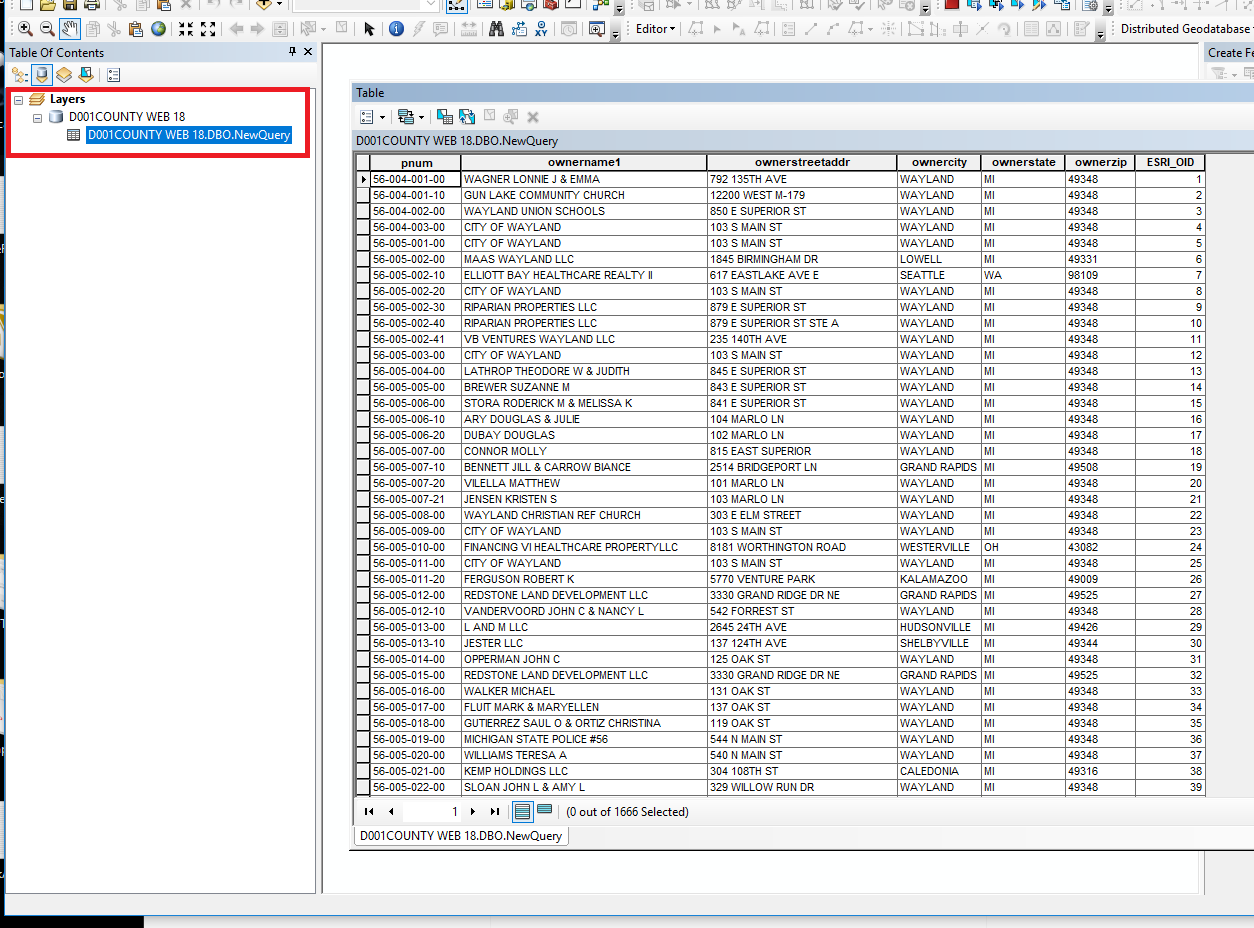
\includegraphics[width=.95\textwidth]{QueryResultsTable.PNG}
\caption{Query Results Table}
\end{figure}
\clearpage
\end{document}
